\documentclass[a4paper,11pt]{article}

\usepackage[utf8]{inputenc}

\usepackage{minted}
\usepackage{graphicx}

\begin{document}


\title{
    \textbf{Sorted report}
}
\author{Jonathan Karlsson}
\date{Fall 2023}

\maketitle

\section*{Introduction}
This assignemnt was to create a binary search algorithm and then comparing it to a linear search algorithm. The task also
included creating a special algorithm using pointers for finding duplicates between two different arrays, and then comparing the speed of this algorithm with the 
linear and binary search. 


\section*{Implementation}
\subsection*{Binary search}
: in code exampels means that part of code that is not shown in the current example.\\ \\
The binary search consisted of multiple if statements that are only possible when the array is sorted. The algorithm starts by setting 
a first and last variable where the first is the start of the array and the last is the end. After that a while loop is run. Inside the 
while loop the first thing that is done is figuring out the midpoint between the first and last element and saving that as index. Then the first
if statement is checked which checks if the element has been found and if so break the loop.
\begin{minted}{java}
int first = 0;
int last = array.length-1;
while (true) {

    int index = (last+first)/2 ;
    if (array[index] == key) {
        break;
}
    :
    :
}
\end{minted}
After the first if statement is checked, the second if statement is checked, which checks if the key is larger than the element the index is pointing to,
if it is the first gets changed to the element ahead of the index and the loop continues to the next iteration.
\begin{minted}{java}
while (true) {
    :
    :       
    if (array[index] < key && index < last) {
        first = index+1;
        continue;
    }
    :
    :
}
\end{minted}
The final if statement checks if the key is smaller than the current element, if it is the last is moved to one lower than the index, and the loop continues. Finally if none of the 
if statements were true, the element did not exist and false is returned, if the element was found the loop would have been broken in the first if statement and then true is returned.
\begin{minted}{java}
while(true) {
    :
    :
        if (array[index] > key && index > first) {
        last = index-1;
        continue;
}
return false;

}
return true;  
\end{minted}
\subsection*{Duplicates}
The check for duplicates was made in three different ways. The first way was to use the linear search algorithm and just go through every element in the first array
and search the second array for that element. If the element is found it is added to an ArrayList.
\begin{minted}{java}
    ArrayList<Integer> duplicates = new ArrayList<Integer>();
    for (int elem : arrayone) {

        if (Linear.search(arraytwo, elem))
            duplicates.add(elem);

        }
    return duplicates;    
\end{minted}
The second way to solve the problem was to use binary search. This was done in the same way as the linear search except for the fact that binary search
is used instead. 
\begin{minted}{java}
    ArrayList<Integer> duplicates = new ArrayList<Integer>();
    for (int elem : arrayone) {

        if(Binary.search(arraytwo, elem))
            duplicates.add(elem);

    }
    return duplicates;
\end{minted}
The final way to check for duplicates was using a special algortihm with pointers, which as with binary search only works if the array is sorted. This algorithm is 
a bit more complicated compared to the prevous two as it doesn't just use a standard search algorithm to find the duplicates, instead two indexes are created. Then if statements are looped until 
one of the arrays run out of elements. If the 
element at the index for arrayone also known as index1 is larger than the element at the index of arraytwo also known as index2, index2 is increased. If the elements are the same 
the duplicate is saved to an ArrayList as in the previous solutions but index1 is also increased. Finally if the element in index2 is larger than the element in index1, index1 is increased. 
\begin{minted}{java}
    int index1 = 0;
    int index2 = 0;
    ArrayList<Integer> duplicates = new ArrayList<Integer>();
    while(index1 < arrayone.length && index2 < arraytwo.length) {
        if (arraytwo[index2]<arrayone[index1]) {
            index2++;
        }
        else if(arraytwo[index2]==arrayone[index1]) {
            duplicates.add(arrayone[index1]);
            index1++;            
        }
        else if (arraytwo[index2]>arrayone[index1]) {
            index1++;
        }
    }
    return duplicates;    
\end{minted}

\section*{Benchmark}
\subsection*{Search algorithms}
The benchmark for the two search algorithms were written such that each algorithm would search for 10000 different elements 1000 times 
in a n sized array and then the best time for that algorithm and array size would be saved. Due to the fact that the
linear seach is too slow it is only benchmarked for n is lower than 100000. The results from the benchmark can be found in the table below.
Some rows were removed from the table to shrink its size, the full table can be found at the end in the full tables section.
\begin{table}[h]
    \begin{center}
    \begin{tabular}{l|c|c}
    \textbf{n} & \textbf{linear ({\textmu}s)} & \textbf{binary ({\textmu}s)}\\
    \hline
    100  &    180 &    270 \\
    200 &    337 &    321\\
    1600 &    2539&    490 \\
    10000 &    15721&    615\\
    128000000 &    &    4849\\


    \end{tabular}
    \caption{The results of the benchmark for the different search algorithms}
    \label{tab:table1}
    \end{center}
\end{table}
\subsubsection*{}
A graph for the benchmark was also created. This shows that the linear search is closest to a linear function while
the binary search is closest to a log function.
\begin{figure}[h]
    \centering    
    
    \scalebox{0.35}{% GNUPLOT: LaTeX picture with Postscript
\begingroup
  \makeatletter
  \providecommand\color[2][]{%
    \GenericError{(gnuplot) \space\space\space\@spaces}{%
      Package color not loaded in conjunction with
      terminal option `colourtext'%
    }{See the gnuplot documentation for explanation.%
    }{Either use 'blacktext' in gnuplot or load the package
      color.sty in LaTeX.}%
    \renewcommand\color[2][]{}%
  }%
  \providecommand\includegraphics[2][]{%
    \GenericError{(gnuplot) \space\space\space\@spaces}{%
      Package graphicx or graphics not loaded%
    }{See the gnuplot documentation for explanation.%
    }{The gnuplot epslatex terminal needs graphicx.sty or graphics.sty.}%
    \renewcommand\includegraphics[2][]{}%
  }%
  \providecommand\rotatebox[2]{#2}%
  \@ifundefined{ifGPcolor}{%
    \newif\ifGPcolor
    \GPcolortrue
  }{}%
  \@ifundefined{ifGPblacktext}{%
    \newif\ifGPblacktext
    \GPblacktextfalse
  }{}%
  % define a \g@addto@macro without @ in the name:
  \let\gplgaddtomacro\g@addto@macro
  % define empty templates for all commands taking text:
  \gdef\gplbacktext{}%
  \gdef\gplfronttext{}%
  \makeatother
  \ifGPblacktext
    % no textcolor at all
    \def\colorrgb#1{}%
    \def\colorgray#1{}%
  \else
    % gray or color?
    \ifGPcolor
      \def\colorrgb#1{\color[rgb]{#1}}%
      \def\colorgray#1{\color[gray]{#1}}%
      \expandafter\def\csname LTw\endcsname{\color{white}}%
      \expandafter\def\csname LTb\endcsname{\color{black}}%
      \expandafter\def\csname LTa\endcsname{\color{black}}%
      \expandafter\def\csname LT0\endcsname{\color[rgb]{1,0,0}}%
      \expandafter\def\csname LT1\endcsname{\color[rgb]{0,1,0}}%
      \expandafter\def\csname LT2\endcsname{\color[rgb]{0,0,1}}%
      \expandafter\def\csname LT3\endcsname{\color[rgb]{1,0,1}}%
      \expandafter\def\csname LT4\endcsname{\color[rgb]{0,1,1}}%
      \expandafter\def\csname LT5\endcsname{\color[rgb]{1,1,0}}%
      \expandafter\def\csname LT6\endcsname{\color[rgb]{0,0,0}}%
      \expandafter\def\csname LT7\endcsname{\color[rgb]{1,0.3,0}}%
      \expandafter\def\csname LT8\endcsname{\color[rgb]{0.5,0.5,0.5}}%
    \else
      % gray
      \def\colorrgb#1{\color{black}}%
      \def\colorgray#1{\color[gray]{#1}}%
      \expandafter\def\csname LTw\endcsname{\color{white}}%
      \expandafter\def\csname LTb\endcsname{\color{black}}%
      \expandafter\def\csname LTa\endcsname{\color{black}}%
      \expandafter\def\csname LT0\endcsname{\color{black}}%
      \expandafter\def\csname LT1\endcsname{\color{black}}%
      \expandafter\def\csname LT2\endcsname{\color{black}}%
      \expandafter\def\csname LT3\endcsname{\color{black}}%
      \expandafter\def\csname LT4\endcsname{\color{black}}%
      \expandafter\def\csname LT5\endcsname{\color{black}}%
      \expandafter\def\csname LT6\endcsname{\color{black}}%
      \expandafter\def\csname LT7\endcsname{\color{black}}%
      \expandafter\def\csname LT8\endcsname{\color{black}}%
    \fi
  \fi
    \setlength{\unitlength}{0.0500bp}%
    \ifx\gptboxheight\undefined%
      \newlength{\gptboxheight}%
      \newlength{\gptboxwidth}%
      \newsavebox{\gptboxtext}%
    \fi%
    \setlength{\fboxrule}{0.5pt}%
    \setlength{\fboxsep}{1pt}%
    \definecolor{tbcol}{rgb}{1,1,1}%
\begin{picture}(7200.00,5040.00)%
    \gplgaddtomacro\gplbacktext{%
      \csname LTb\endcsname%%
      \put(1210,704){\makebox(0,0)[r]{\strut{}$1$}}%
      \put(1210,1161){\makebox(0,0)[r]{\strut{}$10$}}%
      \put(1210,1618){\makebox(0,0)[r]{\strut{}$100$}}%
      \put(1210,2076){\makebox(0,0)[r]{\strut{}$1000$}}%
      \put(1210,2533){\makebox(0,0)[r]{\strut{}$10000$}}%
      \put(1210,2990){\makebox(0,0)[r]{\strut{}$100000$}}%
      \put(1210,3447){\makebox(0,0)[r]{\strut{}$1\times10^{6}$}}%
      \put(1210,3905){\makebox(0,0)[r]{\strut{}$1\times10^{7}$}}%
      \put(1210,4362){\makebox(0,0)[r]{\strut{}$1\times10^{8}$}}%
      \put(1210,4819){\makebox(0,0)[r]{\strut{}$1\times10^{9}$}}%
      \put(1342,484){\makebox(0,0){\strut{}$100$}}%
      \put(2122,484){\makebox(0,0){\strut{}$1000$}}%
      \put(2902,484){\makebox(0,0){\strut{}$10000$}}%
      \put(3682,484){\makebox(0,0){\strut{}$100000$}}%
      \put(4463,484){\makebox(0,0){\strut{}$1\times10^{6}$}}%
      \put(5243,484){\makebox(0,0){\strut{}$1\times10^{7}$}}%
      \put(6023,484){\makebox(0,0){\strut{}$1\times10^{8}$}}%
      \put(6803,484){\makebox(0,0){\strut{}$1\times10^{9}$}}%
    }%
    \gplgaddtomacro\gplfronttext{%
      \csname LTb\endcsname%%
      \put(209,2761){\rotatebox{-270}{\makebox(0,0){\strut{}time in µs}}}%
      \put(4072,154){\makebox(0,0){\strut{}n}}%
      \csname LTb\endcsname%%
      \put(2266,3091){\makebox(0,0)[r]{\strut{}linear}}%
      \csname LTb\endcsname%%
      \put(2266,2871){\makebox(0,0)[r]{\strut{}binary}}%
      \csname LTb\endcsname%%
      \put(2266,2651){\makebox(0,0)[r]{\strut{}n}}%
      \csname LTb\endcsname%%
      \put(2266,2431){\makebox(0,0)[r]{\strut{}log(n)}}%
    }%
    \gplbacktext
    \put(0,0){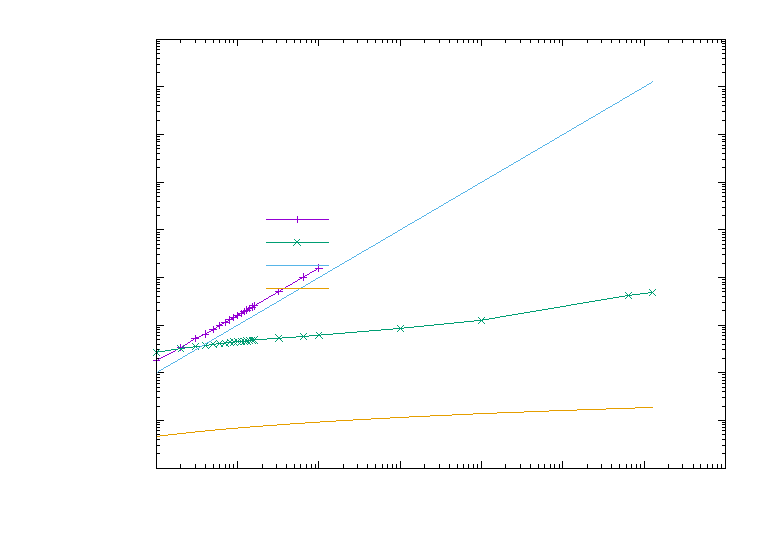
\includegraphics[width={360.00bp},height={252.00bp}]{benching}}%
    \gplfronttext
  \end{picture}%
\endgroup
}
    \caption{Visualization of the times for the two diffent algorithms and basic functions for Visualization}   
    \label{tab:figure1} 
    
    \end{figure}
    


\subsection*{Duplicates}
The duplicate algorithms were benmchmarked in a similar way where first two sorted arrays were created with the selected amount of elements.
Then each algorithm was used 1000 times on the arrays and the minimum time it took was saved. Here the linear search was once again the slowest and therefore got
removed after 25600 elements. A table describing the results can be found below. Full table in full tables section
\begin{table}[h]
    \begin{center}
    \begin{tabular}{l|c|c|c}
    \textbf{n} & \textbf{linear ({\textmu}s)} & \textbf{binary ({\textmu}s)}& \textbf{pointer ({\textmu}s)}\\
    \hline
    100  &5    &    6     &   4       \\
    200 &  12  &    9       &  5      \\
    1600 &449     &    61   &  19      \\
    25600 &113525     &    1030 &   213        \\
    8000000 &    &    435159    &     68416      \\


    \end{tabular}
    \caption{The results of the benchmark for the different duplicate algorithms}
    \label{tab:table2}
    \end{center}
\end{table}
\subsubsection*{}
A graph for the benchmark was also created. Here it is possible to see that the linear search is an $n^2$ function, as it has to go through every n and then do it again for each n in the search itself.
Binary search is $n log n$ for the same reason. The pointer method seems to be faster but following the same path as binary search.
\begin{figure}[h]
    \centering    
    
    \scalebox{0.35}{% GNUPLOT: LaTeX picture with Postscript
\begingroup
  \makeatletter
  \providecommand\color[2][]{%
    \GenericError{(gnuplot) \space\space\space\@spaces}{%
      Package color not loaded in conjunction with
      terminal option `colourtext'%
    }{See the gnuplot documentation for explanation.%
    }{Either use 'blacktext' in gnuplot or load the package
      color.sty in LaTeX.}%
    \renewcommand\color[2][]{}%
  }%
  \providecommand\includegraphics[2][]{%
    \GenericError{(gnuplot) \space\space\space\@spaces}{%
      Package graphicx or graphics not loaded%
    }{See the gnuplot documentation for explanation.%
    }{The gnuplot epslatex terminal needs graphicx.sty or graphics.sty.}%
    \renewcommand\includegraphics[2][]{}%
  }%
  \providecommand\rotatebox[2]{#2}%
  \@ifundefined{ifGPcolor}{%
    \newif\ifGPcolor
    \GPcolortrue
  }{}%
  \@ifundefined{ifGPblacktext}{%
    \newif\ifGPblacktext
    \GPblacktextfalse
  }{}%
  % define a \g@addto@macro without @ in the name:
  \let\gplgaddtomacro\g@addto@macro
  % define empty templates for all commands taking text:
  \gdef\gplbacktext{}%
  \gdef\gplfronttext{}%
  \makeatother
  \ifGPblacktext
    % no textcolor at all
    \def\colorrgb#1{}%
    \def\colorgray#1{}%
  \else
    % gray or color?
    \ifGPcolor
      \def\colorrgb#1{\color[rgb]{#1}}%
      \def\colorgray#1{\color[gray]{#1}}%
      \expandafter\def\csname LTw\endcsname{\color{white}}%
      \expandafter\def\csname LTb\endcsname{\color{black}}%
      \expandafter\def\csname LTa\endcsname{\color{black}}%
      \expandafter\def\csname LT0\endcsname{\color[rgb]{1,0,0}}%
      \expandafter\def\csname LT1\endcsname{\color[rgb]{0,1,0}}%
      \expandafter\def\csname LT2\endcsname{\color[rgb]{0,0,1}}%
      \expandafter\def\csname LT3\endcsname{\color[rgb]{1,0,1}}%
      \expandafter\def\csname LT4\endcsname{\color[rgb]{0,1,1}}%
      \expandafter\def\csname LT5\endcsname{\color[rgb]{1,1,0}}%
      \expandafter\def\csname LT6\endcsname{\color[rgb]{0,0,0}}%
      \expandafter\def\csname LT7\endcsname{\color[rgb]{1,0.3,0}}%
      \expandafter\def\csname LT8\endcsname{\color[rgb]{0.5,0.5,0.5}}%
    \else
      % gray
      \def\colorrgb#1{\color{black}}%
      \def\colorgray#1{\color[gray]{#1}}%
      \expandafter\def\csname LTw\endcsname{\color{white}}%
      \expandafter\def\csname LTb\endcsname{\color{black}}%
      \expandafter\def\csname LTa\endcsname{\color{black}}%
      \expandafter\def\csname LT0\endcsname{\color{black}}%
      \expandafter\def\csname LT1\endcsname{\color{black}}%
      \expandafter\def\csname LT2\endcsname{\color{black}}%
      \expandafter\def\csname LT3\endcsname{\color{black}}%
      \expandafter\def\csname LT4\endcsname{\color{black}}%
      \expandafter\def\csname LT5\endcsname{\color{black}}%
      \expandafter\def\csname LT6\endcsname{\color{black}}%
      \expandafter\def\csname LT7\endcsname{\color{black}}%
      \expandafter\def\csname LT8\endcsname{\color{black}}%
    \fi
  \fi
    \setlength{\unitlength}{0.0500bp}%
    \ifx\gptboxheight\undefined%
      \newlength{\gptboxheight}%
      \newlength{\gptboxwidth}%
      \newsavebox{\gptboxtext}%
    \fi%
    \setlength{\fboxrule}{0.5pt}%
    \setlength{\fboxsep}{1pt}%
    \definecolor{tbcol}{rgb}{1,1,1}%
\begin{picture}(7200.00,5040.00)%
    \gplgaddtomacro\gplbacktext{%
      \csname LTb\endcsname%%
      \put(1210,704){\makebox(0,0)[r]{\strut{}$1$}}%
      \put(1210,1390){\makebox(0,0)[r]{\strut{}$10$}}%
      \put(1210,2076){\makebox(0,0)[r]{\strut{}$100$}}%
      \put(1210,2762){\makebox(0,0)[r]{\strut{}$1000$}}%
      \put(1210,3447){\makebox(0,0)[r]{\strut{}$10000$}}%
      \put(1210,4133){\makebox(0,0)[r]{\strut{}$100000$}}%
      \put(1210,4819){\makebox(0,0)[r]{\strut{}$1\times10^{6}$}}%
      \put(1342,484){\makebox(0,0){\strut{}$100$}}%
      \put(2434,484){\makebox(0,0){\strut{}$1000$}}%
      \put(3526,484){\makebox(0,0){\strut{}$10000$}}%
      \put(4619,484){\makebox(0,0){\strut{}$100000$}}%
      \put(5711,484){\makebox(0,0){\strut{}$1\times10^{6}$}}%
      \put(6803,484){\makebox(0,0){\strut{}$1\times10^{7}$}}%
    }%
    \gplgaddtomacro\gplfronttext{%
      \csname LTb\endcsname%%
      \put(209,2761){\rotatebox{-270}{\makebox(0,0){\strut{}time in µs}}}%
      \put(4072,154){\makebox(0,0){\strut{}n}}%
      \csname LTb\endcsname%%
      \put(2398,2981){\makebox(0,0)[r]{\strut{}linear}}%
      \csname LTb\endcsname%%
      \put(2398,2761){\makebox(0,0)[r]{\strut{}binary}}%
      \csname LTb\endcsname%%
      \put(2398,2541){\makebox(0,0)[r]{\strut{}pointer}}%
    }%
    \gplbacktext
    \put(0,0){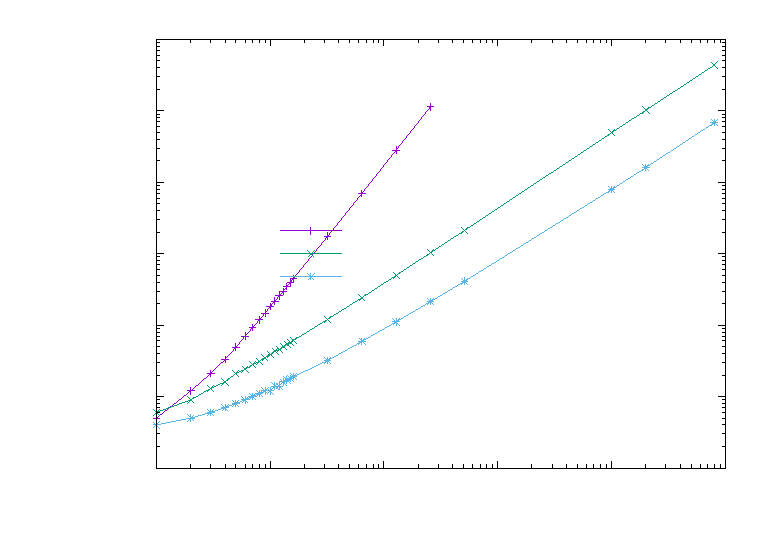
\includegraphics[width={360.00bp},height={252.00bp}]{duplicatestes}}%
    \gplfronttext
  \end{picture}%
\endgroup
}
    \caption{Visualization of the different algorithms for finding duplicates}   
    \label{tab:figure2} 
    

    \end{figure}


\section*{Conclusion}
It is deffinietly easier to search a sorted array. While it is probably faster to just use linear search on an unsorted array as sorting it first will take some time and then actually 
searching through it takes around $log(n)$ time using binary search. However when checking for duplicates it might actually make sense to sort the second array if the first one is already sorted.
This is because the pointer method only seems to be faster than binary search while linear search seems to take $(n^2)$ so if it is possible to find a sort algorithm that when combined with the pointer method is faster
than $(n^2)$ it would be faster to sort the array first.



\newpage
\section*{Full tables}
\begin{table}[ht]
    \begin{center}
    \begin{tabular}{l|c|c}
    \textbf{n} & \textbf{linear ({\textmu}s)} & \textbf{binary ({\textmu}s)}\\
    \hline
    100  &    180 &    270 \\
    200 &    337 &    321\\
    300 &    523 &    354 \\
    400 &    651 &    371 \\
    500 &    804 &    396 \\
    600 &    989 &    409 \\
    700 &    1140 &    418 \\
    800 &    1292 &    436 \\
    900 &    1450 &    441 \\
    1000 &    1610 &    448 \\
    1100 &    1755&    451 \\
    1200 &    1915 &    457 \\
    1300 &    2067 &    463 \\
    1400 &    2225 &    470 \\
    1500 &    2375 &    480 \\
    1600 &    2539&    490 \\
    3200 &    5072&    531 \\
    6400 &    10168&    579 \\
    10000 &    15721&    615\\
    100000 &    &    854\\
    1000000 &   &    1271\\
    64000000 &    &    4202 \\
    128000000 &    &    4849\\


    \end{tabular}
    \caption{The results of the benchmark for the different search algorithms (Full table)}
    \label{tab:table3}
    \end{center}
\end{table}

\begin{table}[ht]
    \begin{center}
    \begin{tabular}{l|c|c|c}
    \textbf{n} & \textbf{linear ({\textmu}s)} & \textbf{binary ({\textmu}s)}& \textbf{pointer ({\textmu}s)}\\
    \hline
    100  &5    &    6     &   4       \\
    200 &  12  &    9       &  5      \\
    300 &21    &    13      &   6     \\
    400 &  33  &    16      &    7    \\
    500 &  49  &    21      &     8   \\
    600 & 70   &    24      & 9       \\
    700 &   92  &    28     & 10       \\
    800 &  118   &    31    &   11     \\
    900 & 147        &  35  &     12   \\
    1000 &182     &    39   &       12 \\
    1100 &217     &    43   &14        \\
    1200 &257     &    46   &  14      \\
    1300 &297     &    50   &    16    \\
    1400 &346     &    54   &      17  \\
    1500 &394     &    57   &18        \\
    1600 &449     &    61   &  19      \\
    3200 & 1752   &    121  &    32    \\
    6400 & 7000     &    243    &  59  \\
    12800 &28194     &    497   &111           \\
    25600 &113525     &    1030 &   213        \\
    51200 &     &    2127       &      411     \\
    1000000 &    &    49231     &         7898  \\
    2000000 &    &    102143    &16052           \\
    8000000 &    &    435159    &     68416      \\


    \end{tabular}
    \caption{The results of the benchmark for the different duplicate algorithms(Full table)}
    \label{tab:table4}
    \end{center}
\end{table}


\end{document}
